\documentclass[draftclsnofoot,onecolumn,letterpaper,10pt]{IEEEtran}
\pagestyle{empty}
\usepackage{geometry}
\usepackage{pgfgantt}
\geometry{textheight=9.5in, textwidth=7in}
\usepackage{float}
\usepackage{graphicx}
\usepackage{algorithm2e}
\usepackage{rotating}

\newcommand{\subparagraph}{}
\usepackage{titlesec}
\setcounter{secnumdepth}{4}
\graphicspath{./images}

\titleformat{\section}[block]{\bfseries\Large}{\thesection}{0.4em}{}
\titleformat{\subsection}[block]{\bfseries\large}{\thesubsection}{0.4em}{}
\titleformat{\subsubsection}[block]{\bfseries\normalsize}{\thesubsubsection}{0.4em}{}
\setlength{\parindent}{0pt}
\renewcommand{\thesection}{\arabic{section}}
\renewcommand{\thesubsection}{\thesection.\arabic{subsection}}
\renewcommand{\thesubsubsection}{\thesubsection.\arabic{subsubsection}}

\titleformat{\paragraph}{\normalfont\normalsize\bfseries}{\theparagraph}{1em}{}
\titlespacing*{\paragraph}{0pt}{3.25ex plus 1ex minus .2ex}{1.5ex plus .2ex}

\author{Connor Yates\\
\texttt{yatesco@oregonstate.edu\\}
\and
Aravind Parasurama\\
\texttt{parasura@oregonstate.edu\\}
\and
Cody Holliday\\
\texttt{hollidac@oregonstate.edu\\}}
\date{\today}
\title{brew.ai Final Report}
\begin{document}
\maketitle

\newpage
\tableofcontents
\newpage

\section{Introduction}

Who requested it?
Why was it requested?
What is its importance?
Who was/were your client(s)?
Who are the members of your team?
What were their roles?
What was the role of the client(s)? (I.e., did they supervise only, or did they participate in doing development)



\section{Client Requirements}
\documentclass[letterpaper,10pt]{article}
\pagestyle{empty}
\usepackage{geometry}
\geometry{textheight=9.5in, textwidth=7in}

\author{Connor Yates\\
\texttt{yatesco@oregonstate.edu}
\and
Aravind Parasurama\\
\texttt{parasura@oregonstate.edu}
\and
Cody Holliday\\
\texttt{hollidac@oregonstate.edu}}
\date{\today}
\title{OpenBrew Problem Statement}
\begin{document}
\maketitle

\newpage

\section{Overview}
Section 2 describes the scope of the requirements for the BrewAI project.
Section 3 defines terms used in the document as well as terms that are normally used when discussing the project.
Section 4 outlines the project in a high level, whereas Section 5 describes the requirements through user stories.

\subsection{Scope}


\section{Definitions}

\section{Introduction}
\section{Overall Description}


\section{Specific Requirements}
As a customer with no brewing experience\\
I want an interface that is simple and streamlined\\
So that I don't have to deal with the technical details of brewing.\\

As a customer\\
I want a brewing device that is easy to take apart\\
So that it is easy to clean\\

As an amateur brewer\\
I want a device that will learn how to make better batches\\
So that I can drink tasty alcoholic beverages.\\

As a hobbyist brewer\\
I want to be able to access advanced brewing settings\\
So that I can precisely manipulate a brewing batch.\\
\\
As an amateur brewer\\
I want the AI to control the brewing hardware\\
So that I don't have to operate the hardware myself\\

As a user\\
I want the data gathered by the device to be saved\\
So that if I unplug the machine I won't lose my past brewing information.\\

As a user\\
I want the device to be waterproof\\
So that the batch doesn't destroy the computer inside.\\

As a user\\
I want the device to detect when a batch has gone bad\\
So that I am not harmed by incorrectly made batches.\\

As a user\\
I want to be able to select what kind of drink I want\\
So that I can have a better variety of drinks that it can make.\\

As a user\\
I want the device to tell me if my inputs would make a bad batch\\
So that I don't waste ingredients.\\

\end{document}

\section{Difference Between Final Product and Client Requirements}



The Client Requirements document was not modified at all during the year, even as we changed the design.
We did however, fail to complete some of the business related requirements from the original document.

\begin{center}
\begin{tabular}{ lll p{0.3\linewidth} }
 \# & Requirement & What happened to it? & Comments \\
\hline
 1 & Microcontroller & Deemed unnecessary and removed from design. & Actuators and sensors  were integrated directly into the Raspberry Pi \\ 
 2 & Business Requirements & Incomplete. & Only the interviews were conducted. \\  
\end{tabular}
\end{center}

\section{Design Document}
\documentclass[draftclsnofoot,onecolumn,letterpaper,10pt]{IEEEtran}
\pagestyle{empty}
\usepackage{geometry}
\geometry{textheight=9.5in, textwidth=7in}

\usepackage{float}
\usepackage{graphicx}
\newcommand{\subparagraph}{}
\usepackage{titlesec}

\titleformat{\section}[block]{\bfseries\Large}{\thesection}{0.4em}{}
\titleformat{\subsection}[block]{\bfseries\large}{\thesubsection}{0.4em}{}
\titleformat{\subsubsection}[block]{\bfseries\normalsize}{\thesubsubsection}{0.4em}{}
\setlength{\parindent}{0pt}
\renewcommand{\thesection}{\arabic{section}}
\renewcommand{\thesubsection}{\thesection.\arabic{subsection}}
\renewcommand{\thesubsubsection}{\thesubsection.\arabic{subsubsection}}



\date{\today}

\title{brew.ai Design Document}

\begin{document}
{\huge\textbf{Senior Software Engineering Design Group 7}}
	\vspace{1cm}

{\Huge\textbf{brew.ai Design Document}}

\vspace{2cm}
\textbf{Connor Yates} yatesco@oregonstate.edu

\textbf{Aravind Parasurama} parasura@oregonstate.edu

\textbf{Cody Holliday} hollidac@oregonstate.edu

\vspace{2cm}
Sponsor

Dale McCauly, College of Business, Oregon State University

\vspace{0.5cm}
	Approved: 

	Version: 1.0


\newpage
\begin{abstract}
	abstract goes here
\end{abstract}
\newpage
\tableofcontents
\newpage
\section{Introduction}
% Perhaps get rid of these subsection titles, and just combine it into one larger section with appropriate paragraph spacings.
% These talk about the Purpose, scope, etc, of this paper.
\subsection{Purpose}
This document describes the architecture and design of the brew.ai project.
It conforms to the IEEE 1016 System Design Document specification, and lays out the design of hardware, learning, and android interfaces for the project.

\subsection{Scope}
Stated generally, brew.ai is a device which automatically brews fermented drinks and improves its performance over time based on user feedback.
This allows for users 
\subsection{Context}
\subsection{Overview}


\section{Glossary}

\section{Stakeholders and Design Concerns}
% Here we list out the design concerns of stakeholders (users, etc...) that we address in this document.
% By laying out the design concerns now, we can address each in turn in the subsequent design sections.

\section{System Overview}

\section{Design Viewpoints}
% Details each design point we choose for this project.
% The tech review had 3 technologies, with 3 choices/investigations for each tech.
% Each of the three technologies chosen should be designed in detail in its own "viewpoint".
% each viewpoint then has its own "view". There can be more than one of these.
% the views describe the specific implementations that each viewpoint covers. Refer to the doc for more info.

\subsection{Abstract Learning from Previous Trials} %connor's
From the inception, a major component of this project is the idea that it can learn from mistakes and experiments, and improve the quality of the brew over time.
This section looks at the system design from the viewpoint of artificial intelligence creation.
From this perspective, all other design choices of the project are abstracted into general data sources and sinks.
To further illustrate this point, the view Impact on Other Designs, in Section~\ref{sec:AIImpact}, will introduce the reader to this viewpoint by describing its view of the rest of the system.
From there, the AI system's internal view of the brew.ai system will be explained and designed.

\subsubsection{Impact on Other Designs}\label{sec:AIImpact}
From the viewpoint of learning, the two other major viewpoints, electronic hardware and user interfaces, have little to no impact upon the operations of the system.
There will be interaction between these viewpoints, but that does not imply the other sections will autonomously impact the operation of the system.

From the AI perspective, the system is built as a thinking agent, with the ability to send and receive signals.
This allows the agent to change the world it sees (input signals) through its actions (sent signals).
The hardware will be the main component the AI will interact with, as it provides information about the world through sensors, and can change the world through its actuators.
From this perspective, the hardware is generalized into the two categories: sensors and actuators.
This is a common view for an agent to take in regards to its interaction with the world~\cite{RussellNorvig}.
A diagram summarizing the agent's view of the system is presented in Figure~\ref{fig:AIsystemDesign}.

\begin{figure}
\begin{center}\label{fig:AIsystemDesign}
	\caption{brew.ai System Heirarchy from the viewpoint of the agent}
	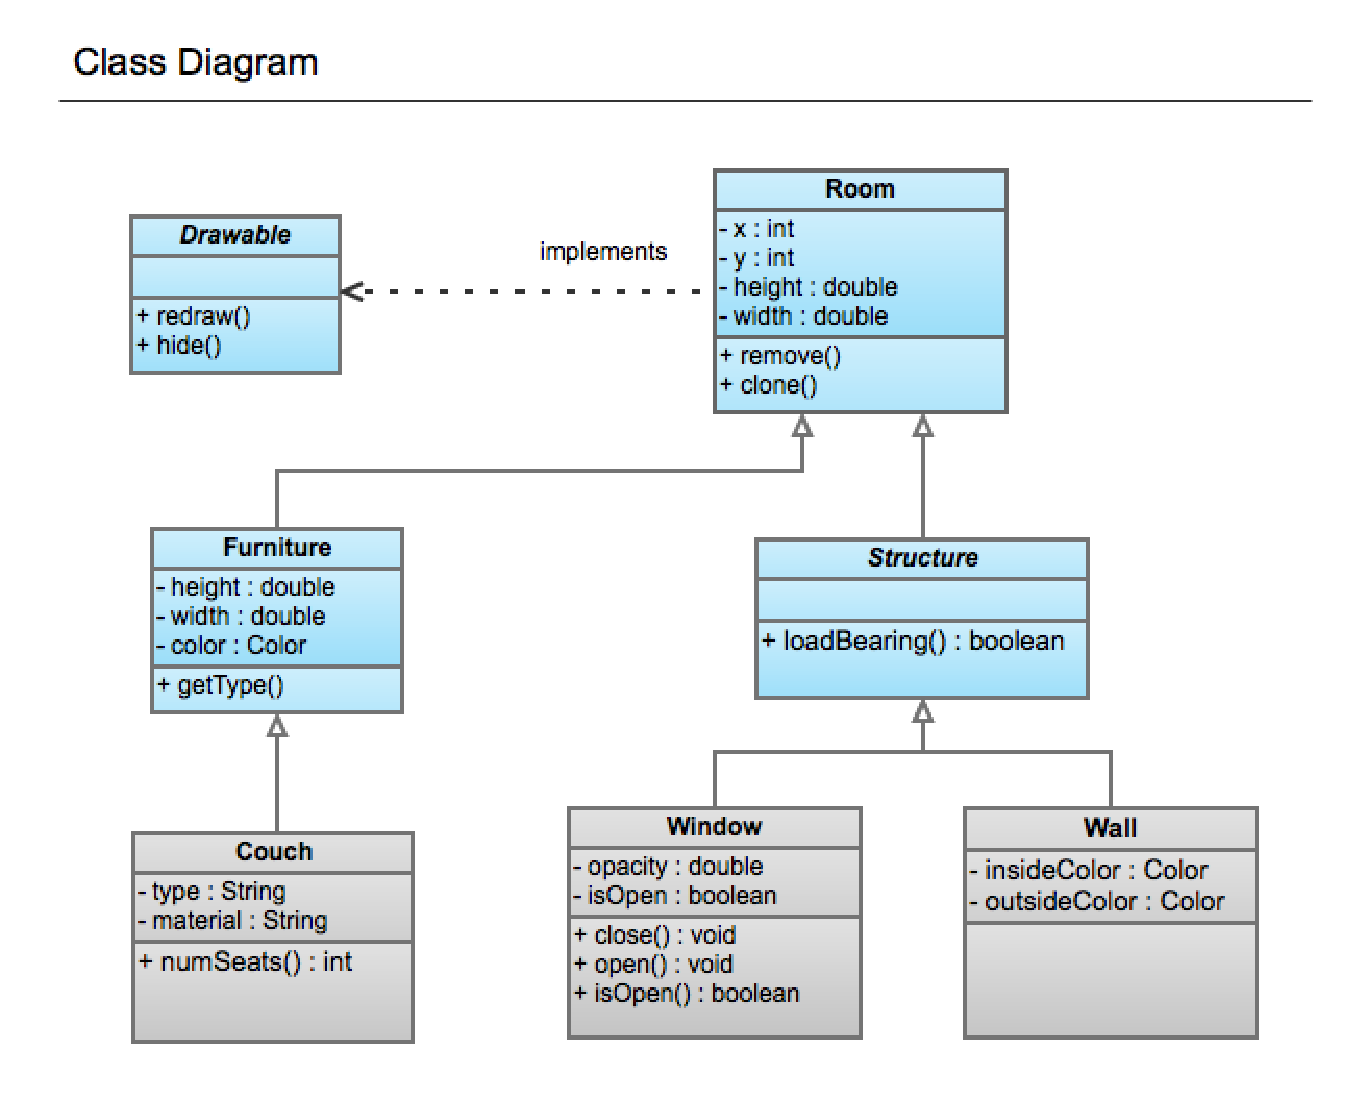
\includegraphics[scale=0.3]{tmp.eps}
\end{center}
\end{figure}

The agent will also view the user interface as source of actuators and sensors, but this will be limited in scope.
The main task of the agent is to brew drinks, not report information to the user.
Therefore, the main decision-making processes will focus on the hardware interaction (reading sensor values, changing temperature levels, etc.) and not on intelligent interaction with the user.
The direct interaction between the user and the AI will be limited to sending statistical information for display, and basic controls such as start-stop controls.

A standard communication layer will be necessary to communicate between the AI, hardware, and interface.
This will be implemented with standard protocols and library packages, such as JSON for interface communication, and byte streams for hardware interaction.
Builtin Python libraries exist for these communication protocols, and subsequently will be used.

\subsubsection{Learning Algorithm} % Replace with design viewpoint name.
% talk about what algorithm I chose.
% Any design considerations that this algorithm requires
% design of this piece, in the context of the project


\subsubsection{Decision Making Structures}
An important aspect of intelligent decision making is the computational structure which allows for decisions to be made.
Neural networks are a classic method of non-linear function approximation which 

\begin{figure}\label{fig:nn}
\begin{center}\label{fig:AIsystemDesign}
	\caption{Proposed Neural Network Structure}
	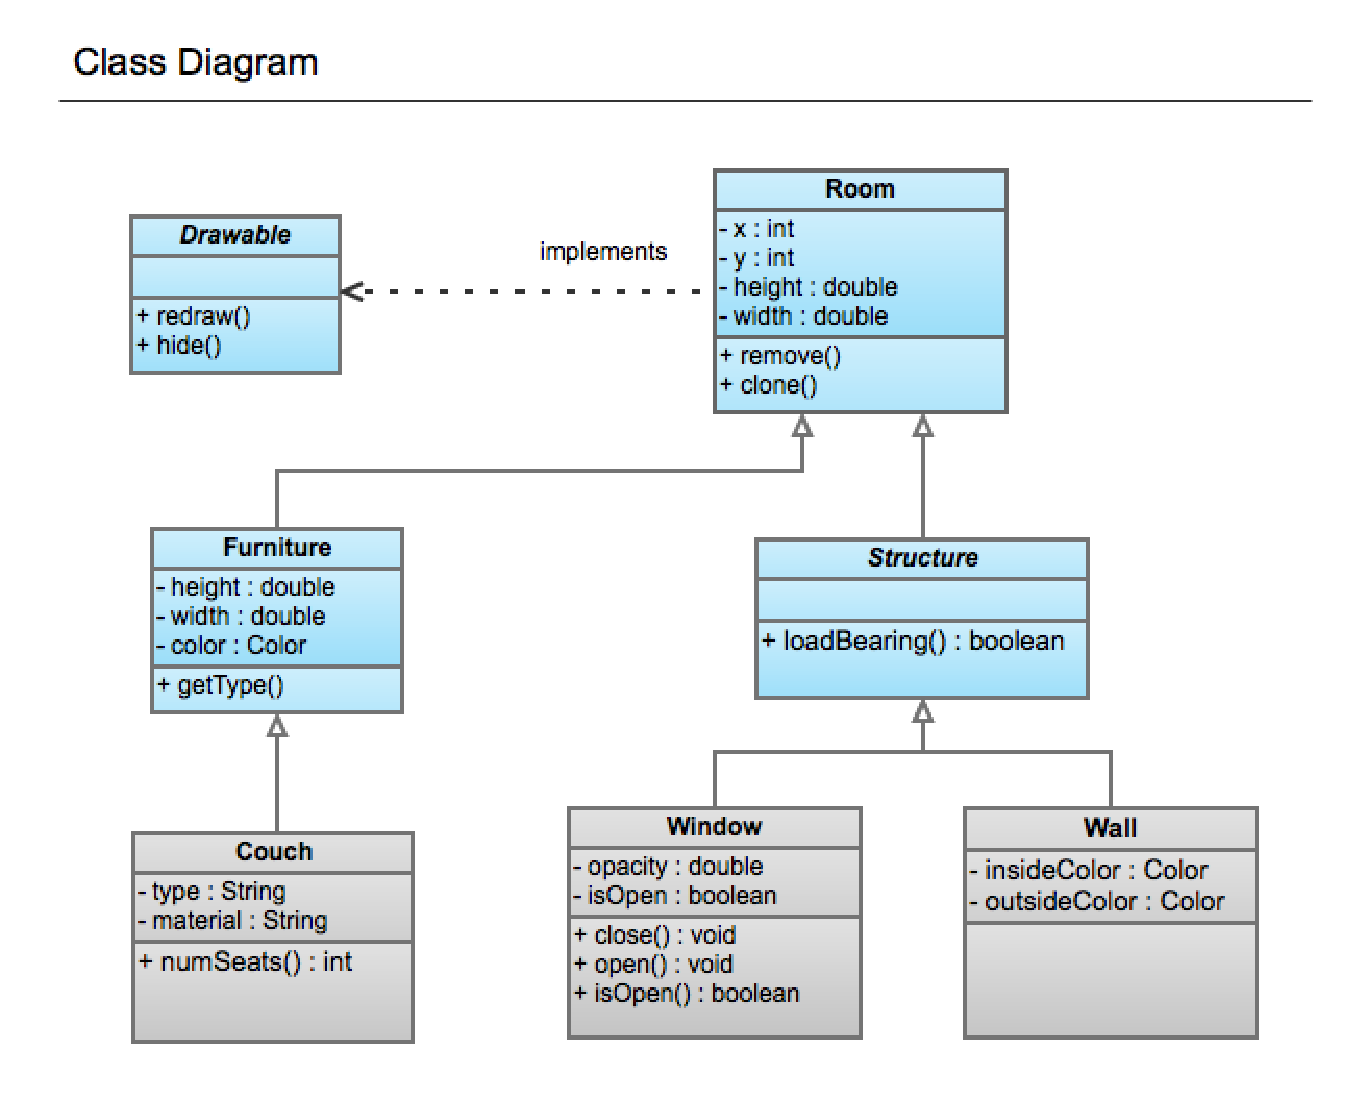
\includegraphics[scale=0.3]{tmp.eps}
\end{center}
\end{figure}

\subsubsection{Library Implementations}

\subsubsection{Overall Learning Structure}
% diagram showing the interaction between the three previous viewpoints

\subsection{Android-Based User Interface Design} %cody's
\subsubsection{Interface Device}

\subsubsection{UI Connection to controller}

\subsubsection{Dataflow to UI}

\subsubsection{Interface layout}


\subsection{Brewing Hardware and Electronic Controls} %aravind's section

\section{Design Rationale}

\section{Testing Details and Timeline}
% Reuse gantt chart for project timeline, and specify where testing would take place in that chart.
% Add details for testing your own components, and potentially testing interactions with other components.

\section{Summary}

% References
\bibliography{design_document}
\bibliographystyle{ieeetr}


\end{document}


\section{How the Design Changed}

During development it was determined that the microcontroller was unnecessary and that the sensors can interface directly with the Raspberry Pi.
This simplified the design and centralized device functionality to the Raspberry Pi.

\section{Tech Review}
zdocumentclass[draftclsnofoot,onecolumn,letterpaper,10pt]{IEEEtran}
\pagestyle{empty}
\usepackage{geometry}
\geometry{textheight=9.5in, textwidth=7in}

\newcommand{\subparagraph}{}
\usepackage{titlesec}

\titleformat{\section}[block]{\bfseries\Large}{\thesection}{0.4em}{}
\titleformat{\subsection}[block]{\bfseries\large}{\thesubsection}{0.4em}{}
\titleformat{\subsubsection}[block]{\bfseries\normalsize}{\thesubsubsection}{0.4em}{}
\setlength{\parindent}{0pt}
\renewcommand{\thesection}{\arabic{section}}
\renewcommand{\thesubsection}{\thesection.\arabic{subsection}}
\renewcommand{\thesubsubsection}{\thesubsection.\arabic{subsubsection}}


\author{Connor Yates\\
\texttt{yatesco@oregonstate.edu\\}
\and
Aravind Parasurama\\
\texttt{parasura@oregonstate.edu\\}
\and
Cody Holliday\\
\texttt{hollidac@oregonstate.edu\\}}
\date{\today}
\title{brew.ai Client Requirements}
\begin{document}
\maketitle

\newpage
\tableofcontents
\newpage
\section{Overview}
This document provides a technical review of three broad topics within the brew.ai project: hardware, user interface, and machine learning.
Each broad topic will be discussed in its own section, preceded by an introduction by the section author.
After the introduction, a review of the potential technologies will be given.
Each broad topic will be divvied into three or more sub-topics, which will address specific technologies that will be combined to address the broad topic of the section.
Finally, each broad topic will have a recommendation about which specific technologies should be used.

\section{Controller Hardware}

\section{User Interface}

\section{Machine Learning \\ -- \textbf{\textit{Connor Yates}}}
\subsection{Introduction}
While a vague title, this section investigates one of the defining features of brew.ai.
In order to create an automated brewing system that not only controls the process in an automated fashion, but can learn from mistakes and improve upon the product, a method of artificial intelligence must be used.
The artificial intelligence that must be imbued in the project has the specific goal of controlling the brewing process.
This is done by sending high level signals such as ``raise temperature'' or ``reduce stir rate'' to the hardware motor controller discussed in Aravind's section.
In order to make these decisions, a continual stream of data from the sensors is fed into the artificial intelligence module, which inform the decision.
Learning will be done in a ``online'' manner, since this allows improvements to the controller policy to happen in between batches \cite{RussellNorvig}.

There are several parts to the artificial intelligence setup for the brew.ai project.
This section will focus on three main aspects: learning algorithm, decision making structure, and preexisting implementations.
It is important to note that these aspects are not mutually exclusive. 
Decisions made in one section may effect the choices in another section.
However, there is still a large degree of freedom between each section, especially with regards to the preexisting software packages that are available.

\subsection{Learning Algorithm}
The class of learning algorithm used is a major choice when setting up the machine learning aspect of the project.
This will dictate how the controller policy will behave while we try to feed it data, which is the most complex part of the machine learning subsection.
\subsubsection{Q-Learning}
Q-learning is a traditional reinforcement learning technique where all possible states and actions are paired up, and a reward mapping between the current state and potential actions can be learned and exploited \cite{SuttonBarto}.
This method is based off a dynamic programming representation of learning, where knowledge from nearby states gets combined into the final value of the state-action pair.
This is important because it creates a solid method of temporal-difference learning \cite{SuttonBarto}, as it becomes possible to associate rewards to series of actions.
As more chains of actions are taken, it can become clear to the agent which actions are preferable in which states.
By learning the action-value function, which returns the most favorable reward at a given state, the agent learns to act optimally within the world.
\subsubsection{Bayesian Modeling with Model Averaging}
Based on the standard Bayesian probabilistic equations, Bayesian modeling uses Bayesian networks as a framework for learning \cite{RussellNorvig}.

While there are different approaches in which Bayesian modeling can be used, the most applicable to our domain is the application known as structure learning \cite{RussellNorvig}.
In this method, machine learning techniques are used to determine the structure of the Bayesian network which best represents the data.

With smaller data sets, such as what I anticipate with this project, a method can be used for Bayesian modeling where multiple models are produced with various dimensionality requirements, and then averaged to create a single model \cite{RussellNorvig}
This allows us to create a better fitting model without needing large amounts of data like other methods would require.

\subsubsection{Deep Learning}
Deep learning is a popular subject in today's media, with the success of projects like AlphaGo grabbing headlines \cite{alphago}.
Conceptually, deep learning focuses on leveraging smart methods of analyzing data to extract high level abstractions and features within complex data sets \cite{Goodfellow-et-al-2016-Book}.
While the technology behind deep learning is impressive, it heavily relies on utilizing massive datasets in order to learn complex, obscure patterns.
This is fundamentally impossible with our project, since we do not have the time nor budget to spend a year gathering data.

\subsubsection{Genetic Algorithms}
Genetic algorithms look at creating powerful solutions to problems by leveraging biologically-inspired techniques \cite{RussellNorvig}.
The concepts of mutation, selection, and genetic crossover have been successfully applied to a variety of state-search problems in the past \cite{RussellNorvig}.
Agent policies, which govern their actions, can be represented as numerical arrays.
The specific transformation for this depends on the model used (ie, neural networks vs state tables).
In either case, genetic algorithms use a population of agent policies which all run and receive a reward.
These rewards are used to calculate the fitness of an policy, which determines how likely the policy is to create offspring and continue to exist \cite{RussellNorvig}.
At the end of each generation of policy performance, the rewards are assigned, fitness is determined, and the creation of new policies begins.
This method is generally modeled after biological reproduction, and can use concepts such as genome crossover and genetic mutation to create new policies to be evaluated.

\subsection{Decision Making Structure}
Some of these methods presented are heavily tied to a specific type of learning algorithm, eg Bayesian networks are mostly only of use when paired with Bayesian models.
However, the differences between these types of structures helps define the state space the learner will operate over.
For example, a neural network can be used as a continuous approximate of a Q-table in continuous reinforcement learning domains.
The decisions present in this section will shape how the problem domain is modeled.

\subsubsection{Neural Networks}
Neural networks are a computational equivalent to neurons within human brains \cite{SuttonBarto}.
The network is made from a series of individual neurons, which are connected in layers.
An individual neuron can be though of as a single linear function: it receives an input signal, applies some weighting and bias, and creates an output signal.
The individual neuron is not incredibly powerful, but when combined in series, they gain the ability to create complex function approximates \cite{SuttonBarto}.

When the weights to individual neurons are set correctly, the connected series of neurons can approximate complex phenomena that would be near impossible to model by hand.
This is one of the major appeals to using neural networks for machine learning tasks.
Additionally, neurons typically receive floating point numbers as input, which does not limit them to discrete domains.
As networks are built, there is no theoretical limit to the number of input or output signals.
This is useful as it allows the network to easily receive each sensor as an input, and send signals to each actuator as output.

\subsubsection{State-Action Table}
State-action tables are a simple method of determine what actions to take.
Simply put, the agent looks at what state it is in - the status of all the information the sensors can provide to the agent.
This state is used as a key which is looked up in the table, where an action is read out.
This action is then acted upon by the agent, and the cycle begins again with sensing.

One issue with this method is that the entire table has to be stored by the agent at all times.
It does not have to be actively loaded into memory constantly, but the table quickly takes up room as the dimensionality of the state grows.
This makes the state-action table representation ill-suited to high-dimensional problems.
However, while this makes this solution infeasible in high-dimensional problems, it creates a strong case for smaller-dimensional problems.
Lookup tables are incredibly quick to access and edit, which allows the agent to have speedy response times in both learning and acting phases.

\subsubsection{Bayesian Networks}
Bayesian networks are directed graphs which represent a probabilistic hierarchy of information \cite{RussellNorvig}.
They allow us to mathematically represent dependencies between fields of information.
For example, the question ``Is it warm in the house?'' is dependent upon the answers to ``Is it summer?'' and ``Do the tenants have a heater?''.
Depending on the status of the answers to the latter questions, we can make a more informed decision about the status of warmth in the house.

Within the context of our problem, a Bayesian network provides the ability to take current sensor readings, and use those to populate a probability table which represents our system.
The dimensionality of that table is determined by the expert in the system (myself, in our case) but the Bayesian network provides the structure on how to fill out the table.
This table is then used to calculate desired probabilities about how much impact given actions would have on the system, which would give us the necessary information to make a decision about the next action to take.

\subsection{Preexisting Implementations}
This section looks at pre-implemented libraries that are available for machine learning routines.
Considerations on memory usage, programming language API, and available functionality are the primary concerns for this sections.
\subsubsection{Keras}
Keras is a high level machine learning suite built for the Python programming language.
\subsubsection{FANN}
\subsubsection{Torch}

\subsection{Recommendation}
\subsubsection{Learning Algorithm}
\subsubsection{Decision Making Structure}
\subsubsection{Preexisting Implementation}


\newpage
\bibliography{tech_review}
\bibliographystyle{ieeetr}


\end{document}


\section{How the Tech Changed}
Besides removing the microcontroller from the design, not much really changed about the technology used.
The learning algorithm, the sensors and actuators, and the android interface pretty much stayed the same.

\section{Weekly Blog Posts}
\section{Weekly Blog Posts}
\subsection{Aravind Parasurama}

\textbf{2016-10-14}

This week, we got the GitHub repository running, with the concerned parties being added as collaborators. Initial stages of design are being completed, as we now have an abstract as well as descriptions of the problem and our solution. The team also met with Dale, to get a better idea of what the Austin Enterpreneurship Program expects from this project. Continuing forward, the hardware implementation of the project needs to be designed and built so that we can start writing and optimizing software. All in all, the project is continuing well.

\textbf{2016-10-21} 

This week, we received feedback on our project proposals. Over the next week, we will have to refine our proposal and have it further evaluated by Dale. We will begin making mead samples this weekend.

\textbf{2016-10-30} 

This week I set up the web hooks for waffle.io, and we got a few documents submitted. Career week was busy, but I met some very interesting companies, and got to network with some very great people. Next week, we'll be updating our requirements doc in anticipation of the final due date this Friday. We'll need to set up a meeting with Dale to get an autograph and to update him with the project, and we'll need to start doing some market research as Dale requested. There's plenty of breweries in Corvallis, so we'll start there. 

\textbf{2016-11-04} 

This has been a busy week with interviews, the GRE, coursework and updating the requirements document. Next week should be just as busy.

\textbf{2016-11-11} 

This is a late update. Last week was very busy, and we managed to get out documents polished for submission. This week will involve working on the tech review and design documents.

\textbf{2016-11-18} 

Finished revising Tech Review. Thanksgiving holiday next week.

\textbf{2016-11-25} 

Starting design document. Finishing it next week.

\textbf{2017-04-07} 

Working on setting up meeting times, and starting test brews.

\textbf{2017-04-14} 

Resuming work from last term on second hardware prototype, updating some GitHub docs. Ordered parts for the second device.

\textbf{2017-04-21} 

Continuing work on second hardware prototype. Arrived parts go in the device, some calibration stuff happens. Worked on poster.

\textbf{2017-04-28} 

Working on poster and hardware prototype. Test brew was a partial success, fixed sensor issues and began another one.


\textbf{2017-05-05} 

Toss the case design for the second device, replace with a repurposed old heat-stirrer. Configure Ph sensor to work.

\textbf{2017-05-12} 

Work on the midterm report, prepare for expo. CAD design some extra box parts, finish up other work with the second device.

\textbf{2017-05-19} 

Expo week. Turned in midterm report, prepared projects for expo, presented at expo.

\textbf{2017-05-26} 

 If you were to redo the project from Fall term, what would you tell yourself?
Don't put a computer above large evaporating masses of liquid. Also, do the progress reports winter term.

 What's the biggest skill you've learned?
Designing and redesigning effective hardware prototypes to make brewing hardware.

 What skills do you see yourself using in the future?
Github and communication skills that I have learned over the course of this term will come in handy over the course of my career.

 What did you like about the project, and what did you not?
I liked learning about brewing, and designing a cool device using new technology that nobody had used for this purpose yet. There was continually new interesting things to learn, and I have had some fun converstaions at interviews because of this project. On the flip side, desigining and building physical hardware prototoypes to test brew with was a time-consuming challenge. There were many different factors that could affect the success of a brew, and the hardware had to conform to all of them while also featuring the functionality brew.ai needed. The process of making these prototypes got pretty frustrating at times.

 What did you learn from your teammates?
I learned cool stuff about how reinforcement learning works, and how to communicate effectively with other software engineers. I also picked up bits of knowledge on Linux and Android development and administration.

 If you were the client for this project, would you be satisfied with the work done?
Yes! The project successfully brews, learns, puts on an interesting show at Expos, and looks good while doing it.

 If your project were to be continued next year, what do you think needs to be working on?
Refined hardware prototypes, extended brew testing, and parallel brews using cloud technology are three key features that brew.ai could use development on if it were continued next year.

\subsection{Connor Yates}

\textbf{2016-10-14} 

Apart from coming down with a nasty cold this week, things seem to be going well. Getting into the groove of things with the group has been good, and our hardware is beginning to be assembled. I feel like this was a good start for the project. Everything got done that needed to be completed, so it certainly could have gone worse!
Getting the GitHub wiki to work isn't the most graceful thing, but I'll keep working on it until it looks the way I want it to. Additionally, as hardware starts to roll in, we will be able to assemble some initial prototypes for our hardware implementation.

\textbf{2016-10-21} 

This week didn't see much action. Rather, there were some minor tests with the GitHub wiki, and some planning for hardware implementations to try out this weekend. Additionally, we have started working on the revisions for the project description, and will get those approved by Dale next week. Next week will also see the writing of the second assignment,the requirements document.

\textbf{2016-10-30} 

The main contribution for this week was the completion of the rough draft of the requirements document.
In the coming week, I look to refine the document within our group, and with our sponsor, as well as begin hardware tests with the brewing setups, and start researching and choosing electronics components to use.
(This update comes a bit late, mainly due to a busy schedule with midterms this week).

\textbf{2016-11-04} 

Well, this week has been hellishly busy between classes and paper writing for my research lab.
The progress on the requirements document came up way to close to the deadline, since peoples schedules were out of synchronization.
I think a long meeting for our group is needed in the near future to rigorously structure how we will add issues, handle pull requests, and allocate our man-hours to effectively make steady progress on the project. 

\textbf{2016-11-11} 

Another late update...
I suppose this has taught me to set a specific time/day to do these, since relying on "after class on friday" doesn't work when there's no class Friday.
This week we divided up the tasks for the technical report. I'll be focusing on the learning aspect, and most likely dividing this section into the three subsections of learning algorithm, decision making architecture, and input structure/learning rate.
Entirely mutually exclusive, and choices in one section may need to be taken into consideration in other sections.

I also have pictures of our current brewing setup, which I will post up here once I figure out a good method of hosting the images.

\textbf{2016-11-18} 

This week, my work on this class was focused on the tech review document. Due to unforeseen circumstances in other classes, the tech review needed extra time to be completed, hence its completion being on Tuesday morning. 
This next week, I want to start in on the final paper for this class by co-opting the previous work we have into the final document. 
Hopefully this paper will go more efficiently than the previous work.

Additionally, now with the tech review completed, I think the time for finalizing and acquiring the hardware has come. This will allow us to work on building the prototype over winter break and begin to record training data. The four weeks of break is too great of a data-gathering opportunity to pass up.

\textbf{2016-11-23} 

I'm publishing this update a little early this week, in anticipation of the holiday.
This week so far hasn't seen any direct progress, aside from setting up some issues in the issue tracker.

The design document is the next deliverable, and as such should take the main priority for this project at the moment.
I plan on working on the document on the 26th, and making sure everyone contributes their parts by Tuesday. I want to have a reviewable draft to Dale by either Tuesday or Wednesday, to give us time to review the document and make any necessary edits.

Sticking to this plan is essential for maintaining progress in this class, as well as ensuring adequate progress in my other classes term projects. As such, I will stick to this plan to the best of my abilities.

\textbf{2016-12-01} 

With the design document fully in progress, I decided to take a break to write this update.
We met with Dale this afternoon, and discusses the progress we made on the design document. There's plenty of time to finish the document before noon tomorrow, and I feel we are in a good place to get it done. The tasks we have left are:
- Finish filling out our respective sections. For me, this entails:
  - Writing up the designs of Q-learning algorithm, the state/action sets, and NN approximator.
  - Create diagrams showing the designs of the agent relationship, NN structure, and agent structure.
  - Discuss some of the testing structures I can use for the agent.
- Review and edit document.
- Test on the server
- Get signatures
- Turn in
- Sleep

And with all of that, our design document will be finished on time.

\textbf{2017-01-20} 

This week we had our first few meetings of the term, both with Frank and Dale. Aravind was out of town for job interviews, but Cody and I were able to make meetings, and set up a weekly time (Monday's after our meeting with Dale) where we can meet as a group to work on the development of the project as a synchronous team. 
After our meeting with Dale, we look to perform two interviews of potential customers in the coming week. This will serve as the start of the interview process, and will allow us to review and reform our interview process as we gather more information from different people. This is a bit of a slow start to the term, but I expect things to pick up quickly.

\textbf{2017-01-23}

AAH! The term started, and it seems I needed to get back into the swing of things more quickly.

This week saw some snow, and a really early class time for the main lecture. I really appreciate not having to go to it constantly this term...

This week we also worked on setting up regular meeting times with Dale and Frank, so that next week we will be able to start back in on the regular, in-person, communication.

\textbf{2017-01-27}

This week became lost time, as I became pretty sick during the later part of the week.
That caused several issues, mainly by building up the stack of work I need to finish apart from capstone (which unfortunatly pushed this update back).
As such, I am having trouble finding time to sit down and work on the AI side of the project.
We've completed 3 of our minimum 5 interviews so far, so we are making some progress on that end.
The interviews have been helpful, especially in seeing how most people interested in a product like this want decent temperature control.
This helps point toward a major area we can focus on in this prototype.

It looks like acquiring hardware is taking a while, but I'm not sure why thats the case.
If that trend holds, it could be disasterous for the completion of the project.

I would definitely say that the project is in a slump right now, and we need to make a concentrated effort to break out of it.

For the upcoming week, my main goal is to sit down by Thursday and finish a working implementation of the approximated Q-learning algorithm.

\textbf{2017-02-03} 

Most of this week's progress has been delayed untill tomorrow (Saturday) as I had two midterms this week.
Even so, there is progress completing more interviews, which is always good, and concrete steps in what needs to happen next.
I am finishing up my week's interview tomorrow, as well as completing a majority of the first iteration of the AI development.
With the coming week, we need to continue our code development, as well as finish off some of the expo-related tasks, including a group leader to handle those.
I have good hopes for our week at the moment, but those hopes remain to be validated at our next meeting.

\textbf{2017-02-10} 

This week my main focus has been on taking care of the AI, and the tasks as the team captain. 
Unfortunatly, I had some work obligations come up in the middle of the week, causing some delays in finishing everything I wanted to finish. Luckily, I'll have time this weekend to finish up the AI, and I aim to do all of the initial OneNote work this evening.
Things are getting done on the project, which is reassuring, but finding time to sit down and work on the project in the middle of a busy term is quite difficult.
But, all I can do is keep pushing forward and put in as much work as I can, making sure to finish things as quickly as possible.

\textbf{2017-02-17} 

This week was writing week! I finished up the OneNote assignment, organizing and doing the document review process.
The OneNote system seems interesting, but I honestly prefer Git and LaTeX. I also use Linux exclusivly, so using a Microsoft web app is a bit morally sickening...
This week I also spent a bunch of my time working on research projects outside of the class, working to help complete a journal paper. This helped cause the need to look for an extension on the presentation, as well as my entire Friday being dedicated to a grad school event. Quite the week, and the weekend will be just as busy... But we just gotta march on.

As of this writing, I've finished up my writing for the progress report, so now all that remains is to edit the sections together, and then it is done. The plan is that once this is finished, we can show it as the sufficient progress to get the extension on the presentation. 

\textbf{2017-02-24} 

This week was a bit uneventful, but the class this week for practicing pitching was actually really useful.
Seeing what Kevin had to say about our presentation was pretty eye opening, since I honestly hadn't considered people *not* being intrigued by a homebrewing device. But this will make the expo day go better, so its very useful.

I am making good progress on the AI code, and if I can find the time this weekend, I believe I can finish it.

\textbf{2017-03-03} 

This week I set up Keras and Theano on the Raspberry Pi B+, the instructions for which I have replicated [here](https://github.com/bitschift/brew.ai/wiki/Setting-up-the-Pi).

I also signed up the group for expo, so that is out of the way. Luckily the next steps as the team captain do not seem to start until next term. 
With the Q learning algorithm written, this weekend I will be working on implementing a simulator to generate a test set of training data for the AI.

I organized a group meeting earlier in the week, where we were able to meet and get some more work done. I'll continue doing this throughout the life of the project, since my code side is finishing up quickly. But I am getting frustrated with the rate of progress on this project, and I am worrying about the fate of the project.

\textbf{2017-03-10} 

Whoopse, I had a test yesterday and I forgot to post this. 
This last week I've been working to organize the group through our last development push for this term.
So the things we need to finish up are:
* Complete analysis on Q-learning agent
  * Test simulator
  * Analyze results and make into a short presentation
* Complete hardware integration
  * Lasercut/3D print new housing structures after redesign to avoid water vapour near the pi.
  * Get Pi talking to a phone app via bluetooth, and have it send the data in real time so the graphs can be redrawn.
  * Assemble product, and show a full working stack. To show the full stack, we will
     * Show a series of prepicked commands can be sent to the hardware from the pi, and the data being observed can be sent to the phone.
     * Show an untrained AI on the pi can be integrated and send commands to the hardware.
    
    The idea of this is to show a fully working product, with the major functionality set up. The untrained AI is used in place while we gather data and perform the offline training. For functionality purposes, all we need to show is decisions being made, and user based reward-learning occuring. Further along, we can provide an AI which actually makes good decisions.

We are meeting up on Sunday (\textbf{2017-03-12}) to finish the integration of the above tasks, and possibly record video of the working prototype.

The simulator is finished, and I am able to run tests which show learning occuring by looking at the increase in system reward (with a higher reward equating to a better brew). Tomorrow or Monday evening, I'll prepare that into a short presentation to cleanly show the working Q-learner.

On the administrative side, we need to
* Review design documents now that the Teensy is not being used.
* Create the rough draft of the poster so we can turn that in.

\textbf{03-23-2017}

It appears that in the joy of the last day of classes, I forgot about the final update... Silly me.

Anyways, this week we had final meetings with Dale, our sponsor, and Frank. Through these, we demonstrated a completed prototype which has full communiction of information: General commands from the phone, specific commands from the AI, and hardware control down to the physical actuators and data from the sensors back to the AI and phone. It sure is cool to see it all working!

In the immediate future, the next steps are to create the final progress report for winter term and the group presentation of the project.
In the larger scale, we will attempt to create a larger, second prototype in the coming weeks which not only will have a larger brewing chamber, but will have room for additional sensors to connect to the Pi.

\textbf{2017-04-16} 

Of note, the first half of this week I was in Canada visiting other schools.
This last week I met with Kirsten on Friday morning to discuss our poster, and got some good feedback. I'll be implementing that in our poster this evening.
I've also continued to arrange the weekly work times on Thursdays where we meet and discuss/work on the project.

In addition to this, I've been reworking the Python code on the RPi, to make it clean and better organized. This has been going well, as it's not hard to make Python look nice when you follow the language standards.

For this next week we will be finishing gathering data from the brewing device, as well as continuing to rework the current code/product and make it look nice for expo.

\textbf{2017-04-28} 

This week we mainly worked on the poster and getting everything tied up cleanly. There are only a few minor edits to the code to upload to github this weekend, so things look easy on that end. There's not much news honestly, since things have wrapped up nicely here toward the end. After expo, the document writing should go smoothly, and pose liffle difficulty to finishing the course.

\textbf{2017-05-26} 

This is the post-expo blog post, so I'll answer the questions in order.

1. If you were to redo the project from Fall term, what would you tell yourself?
Set aside an hour each day in the morning, when everything is quiet, to work on the code development. Development itself doesn't take that much time, so splitting it up each day will probably see the main development done by the midterm mark with ease. 

2. What's the biggest skill you've learned?
Project management, for sure. Making sure the tea operates cleanly and gets all their parts done on time is not easy, and having taken on that roll I found myself challenged in a way I haven't really seen before.

3. What skills do you see yourself using in the future?
I do not see myself using many coding specific techniques or algorithms from this class again. I will probably use Q-learning again, but I've implemented that in the past. Project management would be the main skill where I will be continuing to use it again. I will have larger projects in the future, and keeping them on schedule will always be a non-trivial task.

4. What did you like about the project, and what did you not?
Technically, the project was very fun. I was able to work in Python, an language I am very comfortable with, and it had a cool concept. The most frustrating part of the project was the large ammount of writing associated with it. Writing for large projects is a given, but at many times it felt like there was no major reason behind the writing. Instead, writings in the latter two terms seemed tangential to actual project work.

5. What did you learn from your teammates?
Life gets in the way of people from time to time. It happens to all of us. Subsequently, I learned that when in a magerial role, I should plan for delays in others work just as I plan for them in mine. 

6. If you were the client for this project, would you be satisfied with the work done?
I would say so. We have a working prototype of a product, which can be refined further with a little work. No project of significant scale can be developed in 6 months and be perfect.

7. If your project were to be continued next year, what do you think needs to be working on?
  1. Continued data collection
  2. Further physical refinement
  3. Creation of an end-to-end deplyment system so it works after just being plugged in

\subsection{Cody Holliday}

\textbf{2016-10-14}

This week went well. Our team is competent in writing as well as LaTeX, so the first couple writing assignments were quite quick. Our meeting with our sponsor helped us understand how we are going to incorporate business into the project. This gave us a little more structure in how to go about this project. 

Hopefully next week we can begin our cycles of brewing so that eventually we can provide our algorithm with a god amount of data. Or alternatively work can begin on the device that will be making the mead. I have an arduino that we can use, so we are not held back by getting a microcontroller. 

\textbf{2016-10-21} 

This week was uneventful. We made revisions on our problem statement as well as read about the brewing process. Otherwise not much was accomplished. I was busy with other classes like CS 444.

\textbf{2016-10-30} 

This week was stressful. Plans were made to brew mead, but unexpected surprises came up and we didn't end up going through with it. The requirements document took much longer than expected as not all of us split up the work evenly. Because of this we weren't able to have our document ready for our sponsor meeting, which is very unfortunate. Overall not enough time was spent doing the things we had to do.

\textbf{2016-11-04} 

This week was challenging. Another group member and I had little time for the client requirements document, so the work on revision rested solely on one group member. This was stressful, as we ended up not finishing the document in time for our sponsor meeting. We weren't able to brew this week. It's incredible how much time you can spend doing things and yet not accomplish what you need to do. This sunday we are brewing mead as per our TA's request. 

\textbf{2016-11-11} 

This week we had a successful mead brewing session. Two jars of mead were made. Next week I hope we can ope them up to test their quality and measure our success. We did have some issues with the instructions we were given as they were vague on many of the measurements and times. Either we should use a different set of instructions, or we should request that our current instructions be updated.

\textbf{2016-11-18} 

The past week has been hectic. We successfully completed our tech review and got a better idea of what we have to do for the project. I had issues with work ethic which lead to some increased workload, but we completed it. Next week we should be finished with our first batch of mead as well as have made a significant effort on our design document.

\textbf{2016-11-25} 

Not much happened this week since about half of it was taken up by Thankgiving break. We're looking ahead to next week so that we can have the draft done much earlier than the due date. Hopefully we will have a draft done tuesday or wednesday. At least I think that's when we were thinking. It might be later than that. The batch is still undergoing the brewing process. We should probably go check it out.

\textbf{2016-12-2} 

We successfully completed the preliminary design document, but not without some bumps. I had to rewrite the section on communication between the interface and the controller because my group mates disagreed with my choice. This was frustrating, but I was able to work through it. I hope next week we can finish the progress report in a timely manner.

\textbf{2016-1-27} 

We were able to get two interviews in the past week, one from a coworker of mine and another from Connor's friend. In our meeting with our sponsor he was happy to have found that we conducted these interviews. I have not yet made progress on the bluetooth app communication, but in the coming week I believe that I will. In addition we will interview more people who are less experience with brewing.

\textbf{2016-2-18} 

This last week was one of the least productive weeks I have had personally on this project. With all the events happening in this week from my birthday to Valentines Day, I was not able to bring my project up to alpha standards. However, I was able to lighten my load of work for the term so that I can focus on the project. Next week I pan on having at the least alpha functionality. That means two way Bluetooth and command protocol between the controller and the Android.

\textbf{2016-3-10} 

This past week we outlined what we need to demonstrate for our weekly meeting. I was able to get large dataset communication as well as graphing working between the phone and my computer. I need to pair the phone with the raspberry pi before I can continue working. We are planning on having a separate Bluetooth listener thread that communicates with the main program through a FIFO as well as have continuous updates from the raspberry pi to the Android. I hope to get this completed this weekend.

\textbf{2017-3-21} 

This last week was very productive. I created the layout for the brewing survey, which took a long time. Creating layouts for an app is like making a website, which I actually kind of despise. Learning how to best make a layout is kind of obnoxious as well. Other than that I added functionality to the survey so it sends a value back to the computer that represents what the user wrote in their survey. For the next week I hope to implement the raspberry pi telling the android that brewing has ended, resulting in the android prompting the user about the survey.

\textbf{2016-4-14} 

This last week was good. We determined what we need to do for the rest of the term and what we want to have ready for expo. Since my portion is not as fleshed out as I would like it to be we will have to shoot for something that's a little less than planned. Next week I hope to have the user surveys done so that the AI can learn from user responses.

\textbf{2017-5-25} 

This is the Post-Expo Blog!

1. If I had to redo the project starting fall term, I would tell myself to start on the bluetooth connectivity earlier. Getting that to work was such a hassle and it really kept me from doing more than I wanted to. In addition, I would say to work over winter brewk. It would have saved us much more hassle.

2.The biggest skill I learned was how to learn. This was the first time that I undertook a major project that had an effect on my grade. The pace at which I had to complete my work made me realize how little I usually had to do my homework. I learned how to be interested in learning and how to push myself to do real work.

3. I see myself using my research skills in the future. A lot of effort went into getting bluetooth to work as well as to make the app look good. In addition, some of the design techniques we used are certainly applicable to future projects.

4. I really liked some of the freedom we had. We created this project so we got to define what we wanted. Designing the app was really satisfying, but getting bluetooth connectivity was more than I could have wanted.

5. We worked pretty independently most of the time. I learned some interesting design methods as well as how to mesh communication between two different devices.

6.Well, initially I had a big mental image of what I wanted to make. Now that I have trudged through it all I would be sort of satisfied, but I would understand why it didn't live up to expectations.

7. I think what needs to be worked on is almost everything on my part. The way it acquires data and sends it to the android is completely independent of the main thread. There is nothing to catch disconnection, and if it does disconnect, the device goes into an undefined state where it can't communicate with the android and the main brewing thread is stuck at the end. This is troublesome since brews take months to make, and the user shouldn't be expected to stand there with the app open for months. The Android app is not fully implemented. It needs to query the raspberry pi about previous brews. It needs to have a settings section. The data it collects in the prebrewing state needs to actually be given to the AI to use. There are a lot of things that need to be improved about this project.

\textbf{2017-6-3} 

Not much is left to be done for senior design. We completed the three writing assignments and now all we have to look forward to is the final report. I'm going to finish that by this Saturday since I will be on a trip during finals week in Bend.



\section{Poster}
\newpage
\vfill
\begin{sidewaysfigure}[ht]
\includegraphics[width=\textwidth]{./images/team07.eps}
\end{sidewaysfigure}
\vfill
\clearpage


\section{brew.ai Documentation}

\section{Tech Information Sources}
\subsection{Cody Holliday}
There were only two sites that really helped me with this process: stack overflow and the Android documentation.
Finding information about implementing Bluetooth on a Raspberry Pi was the biggest hassle of the project.
I initially started using an HID Bluetooth dongle, so I looked through the man pages to find out how to use it, but ended up finding out that it had a kernel bug that caused it to malfunction.
I found information to enable normal HCI Bluetooth from a blog post about connecting an Android phone to a Raspberry Pi.
This blog post is on blog.davidvassallo.me.
The order of usefulness is Stack Overflow, Android Documentation, and blog.davidvassallo.me.
The blog is last since it solves a very specific problem, while the others helped with many other problems.

\section{What Did We Learn?}
\subsection{Cody Holliday}
I think overall, I learned how to learn. This year was a struggle for me because I had to push myself to be an independent worker.
I have worked on an independent project before, but I was terrible at it.
I didn't know how to do anything, and I didn't have the drive to learn independently. 
I relied heavily on other people to help me with my work.
But going through Senior Design has really shown me how to manage my time and how to have the drive to work independently.
Working in teams was nothing new to me. However, I did learn how to effectively be part of a team.
That's not something that can be taught outside of a class like this, since most only last ten weeks.
The technical information I learned was not too different than what I learned before.
Sockets and basic programming were normal to me. What was different was enabling Bluetooth on the Pi and learning how activities worked on Android.
Throughout this year I have learned more and more about Linux and how kernel modules work.
Working with Bluetooth allowed me to put some of that knowledge to work.
In much the same way, learning about Android activities and fragments allowed me to use what I learned from my software engineering courses.
The Android activity is like a process. It's big, hefty, and has a lot of functionality.
Fragments are sort of like smaller activities. Their main purpose is to reuse parts of an Android activity to save memory and storage.
If I could do the whole project over again, I would use a framework when developing the app.
I wrote the app in java using Android studio, which is much more difficult than using a framework that does the heavy lifting for you.
That would save so much time and hassle that I would have had to deal with in the later stages of development.


\appendix
\section{Code Listings}
\section{Photos, Etc.}

\end{document}
